% ============================================================================
% EMCH 501: Engineering Analysis I - Assignment 4 (Enhanced Solutions)
% ============================================================================

\documentclass[12pt]{article}

% ============================================================================
% PACKAGE IMPORTS
% ============================================================================
\usepackage{amsmath}
\usepackage{graphicx}
\usepackage{amssymb}
\usepackage{tikz}
\usepackage[margin=1in]{geometry}
\usepackage{setspace}
\usepackage{xcolor}
\usepackage{enumitem}
\usepackage{tcolorbox}
\usepackage{fancyhdr}
\usepackage{lastpage}
\usepackage{booktabs}
\usepackage{array}
\usepackage{colortbl}
\usepackage{pgfplots}
\usepackage{listings}
\usepackage{float}
\pgfplotsset{compat=1.18}

% ============================================================================
% HEADER AND FOOTER SETUP
% ============================================================================
\pagestyle{fancy}
\setlength{\headheight}{14.5pt}
\fancyhf{}

\fancyhead[L]{Page \thepage\ of \pageref{LastPage}}
\fancyhead[C]{EMCH 501}
\fancyhead[R]{JC Vaught}

\renewcommand{\headrulewidth}{0pt}

% ============================================================================
% TIKZ LIBRARIES
% ============================================================================
\usetikzlibrary{shapes.geometric, arrows.meta, positioning, decorations.pathmorphing, patterns}

% --- USC Brand Colors ---
\definecolor{USC_Garnet}{HTML}{73000A}
\definecolor{USC_Sandstorm}{HTML}{FFF2E3}
\definecolor{USC_Black90}{HTML}{565656}
\definecolor{USC_Black10}{HTML}{ECECEC}
\definecolor{USC_Honeycomb}{HTML}{65780B}
\definecolor{tablegreen}{RGB}{230,242,230}
\definecolor{outputbg}{RGB}{245,245,245}

% ============================================================================
% CUSTOM COLORED BOXES
% ============================================================================
\newtcolorbox{stepbox}{
  colback=white,
  colframe=USC_Garnet,
  fonttitle=\bfseries,
  title=Step,
  sharp corners,
  colbacktitle=USC_Garnet,
  coltitle=white,
}

\newtcolorbox{codebox}{
  colback=USC_Black10,
  colframe=USC_Black90,
  fonttitle=\bfseries,
  title=Python Implementation,
  sharp corners,
  colbacktitle=USC_Black90,
  coltitle=white,
}

\newtcolorbox{outputbox}{
  colback=outputbg,
  colframe=USC_Honeycomb,
  fonttitle=\bfseries,
  title=Python Output,
  sharp corners,
  colbacktitle=USC_Honeycomb,
  coltitle=white,
  breakable,
}

\newtcolorbox{resultsbox}{
  colback=white,
  colframe=USC_Honeycomb,
  fonttitle=\bfseries,
  title=Results,
  sharp corners,
  colbacktitle=USC_Honeycomb,
  coltitle=white,
}

% ============================================================================
% CUSTOM QUESTION AND PART COMMANDS
% ============================================================================
\newcommand{\question}[1]{%
  \clearpage
  \vspace{0.5cm}
  {\noindent\normalsize \textbf{#1}}
  \vspace{0.2cm}
  \hrule
  \vspace{0.1cm}
  \hrule
  \vspace{0.3cm}
}

\newcommand{\questionpart}[1]{%
  \clearpage
  \vspace{0.5cm}
  {\noindent\normalsize \textbf{#1}}
  \vspace{0.2cm}
  \hrule
  \vspace{0.1cm}
  \hrule
  \vspace{0.3cm}
}

% Code listing style
\lstset{
    language=Python,
    basicstyle=\ttfamily\small,
    keywordstyle=\color{blue},
    commentstyle=\color{USC_Honeycomb},
    stringstyle=\color{USC_Garnet},
    breaklines=true,
    showstringspaces=false,
    backgroundcolor=\color{USC_Black10},
    numbers=left,
    numberstyle=\tiny\color{gray},
    numbersep=5pt,
}

% Output listing style
\lstdefinestyle{output}{
    basicstyle=\ttfamily\footnotesize,
    breaklines=true,
    showstringspaces=false,
    backgroundcolor=\color{outputbg},
    frame=none,
    numbers=none,
}

% Graphics path
\graphicspath{{figures/}}

% ============================================================================
% DOCUMENT INFORMATION
% ============================================================================

\title{EMCH 501: Engineering Analysis I \\ Assignment 4 \\ \large{Enhanced Solutions with Python Implementation}}
\author{Instructor: Yi Wang, Department of Mechanical Engineering \\ University of South Carolina \\ \textit{Solutions by: JC Vaught}}
\date{Due: December 8, 2025}

% ============================================================================
% BEGIN DOCUMENT
% ============================================================================

\begin{document}

\maketitle
\setlength{\parindent}{0pt}

\setlist[enumerate,1]{label=\arabic*.}
\setlist[enumerate,2]{label=(\alph*)}

% ============================================================================
% TABLE OF CONTENTS
% ============================================================================

\begin{center}
\begin{tcolorbox}[colback=white, colframe=gray!50!black, colbacktitle=gray!20!white,
                  coltitle=black, sharp corners, boxrule=1pt,
                  title=\Large\bfseries Table of Contents]
\begin{tabular}{p{0.82\textwidth}r}
\textbf{Exercise 15.1: Problem 7 (25 pts)} & \\
\quad Part (a): Derivation of Difference Equation \dotfill & \textbf{\pageref{quest:1a}} \\
\quad Part (b): Solution of Poisson Equation \dotfill & \textbf{\pageref{quest:1b}} \\[0.3em]
\textbf{Exercise 15.2: Problem 10 (20 pts)} & \\
\quad Part (a): Finding $\lambda$ \dotfill & \textbf{\pageref{quest:2a}} \\
\quad Part (b): System of Equations \dotfill & \textbf{\pageref{quest:2b}} \\
\quad Part (c): Solving the System \dotfill & \textbf{\pageref{quest:2c}} \\[0.3em]
\textbf{Exercise 15.2: Problem 12 (25 pts)} \dotfill & \textbf{\pageref{quest:3}} \\
\end{tabular}
\vspace{0.2cm}
\end{tcolorbox}
\end{center}

\vspace{0.5cm}

% ============================================================================
% PROBLEM 1: Exercise 15.1 Problem 7 - Part (a)
% ============================================================================

\questionpart{Exercise 15.1: Problem 7 --- Part (a) (25 pts)}\label{quest:1a}

The non-homogeneous form of Laplace's equation is known as Poisson's equation:
\[
\frac{\partial^2 u}{\partial x^2} + \frac{\partial^2 u}{\partial y^2} = f(x,y)
\]
Poisson's equation is commonly used to describe systems involving electric potentials (denoted $u(x,y)$), and $f(x,y)$ can be thought of as the charge density.

\vspace{0.3cm}
\textbf{(a)} Show that the difference equation replacement for Poisson's equation is
\[
u_{i+1,j} + u_{i,j+1} + u_{i-1,j} + u_{i,j-1} - 4u_{i,j} = h^2 f(x,y)
\]

\begin{stepbox}
\textbf{Step 1: Taylor Series Expansion}

To derive the finite difference approximation, we use Taylor series expansions about the point $(x_i, y_j)$.

\textbf{Forward expansion in $x$:}
\[
u(x+h, y) = u + h\frac{\partial u}{\partial x} + \frac{h^2}{2!}\frac{\partial^2 u}{\partial x^2} + \frac{h^3}{3!}\frac{\partial^3 u}{\partial x^3} + \frac{h^4}{4!}\frac{\partial^4 u}{\partial x^4} + O(h^5)
\]

\textbf{Backward expansion in $x$:}
\[
u(x-h, y) = u - h\frac{\partial u}{\partial x} + \frac{h^2}{2!}\frac{\partial^2 u}{\partial x^2} - \frac{h^3}{3!}\frac{\partial^3 u}{\partial x^3} + \frac{h^4}{4!}\frac{\partial^4 u}{\partial x^4} + O(h^5)
\]

Adding these two expansions:
\[
u(x+h, y) + u(x-h, y) = 2u + h^2\frac{\partial^2 u}{\partial x^2} + \frac{h^4}{12}\frac{\partial^4 u}{\partial x^4} + O(h^6)
\]
\end{stepbox}

\begin{stepbox}
\textbf{Step 2: Central Difference Approximation}

Solving for the second derivative:
\[
\frac{\partial^2 u}{\partial x^2} = \frac{u(x+h, y) - 2u(x, y) + u(x-h, y)}{h^2} - \frac{h^2}{12}\frac{\partial^4 u}{\partial x^4} + O(h^4)
\]

Using grid notation where $u_{i,j} = u(x_i, y_j)$:
\[
\frac{\partial^2 u}{\partial x^2} \approx \frac{u_{i+1,j} - 2u_{i,j} + u_{i-1,j}}{h^2} + O(h^2)
\]

Similarly for $y$:
\[
\frac{\partial^2 u}{\partial y^2} \approx \frac{u_{i,j+1} - 2u_{i,j} + u_{i,j-1}}{h^2} + O(h^2)
\]

\textbf{Truncation Error:} The central difference approximation has a truncation error of $O(h^2)$, making it a \textbf{second-order accurate} scheme.
\end{stepbox}

\begin{stepbox}
\textbf{Step 3: Substitution into Poisson's Equation}

Substituting both approximations into $u_{xx} + u_{yy} = f$:
\[
\frac{u_{i+1,j} - 2u_{i,j} + u_{i-1,j}}{h^2} + \frac{u_{i,j+1} - 2u_{i,j} + u_{i,j-1}}{h^2} = f_{i,j}
\]

Multiplying both sides by $h^2$:
\[
u_{i+1,j} - 2u_{i,j} + u_{i-1,j} + u_{i,j+1} - 2u_{i,j} + u_{i,j-1} = h^2 f_{i,j}
\]

Combining the center terms:
\[
u_{i+1,j} + u_{i-1,j} + u_{i,j+1} + u_{i,j-1} - 4u_{i,j} = h^2 f_{i,j}
\]
\end{stepbox}

\begin{resultsbox}
The difference equation replacement for Poisson's equation is:
\[
\boxed{u_{i+1,j} + u_{i,j+1} + u_{i-1,j} + u_{i,j-1} - 4u_{i,j} = h^2 f(x,y)}
\]

This is known as the \textbf{five-point stencil} or \textbf{five-point Laplacian}:
\begin{center}
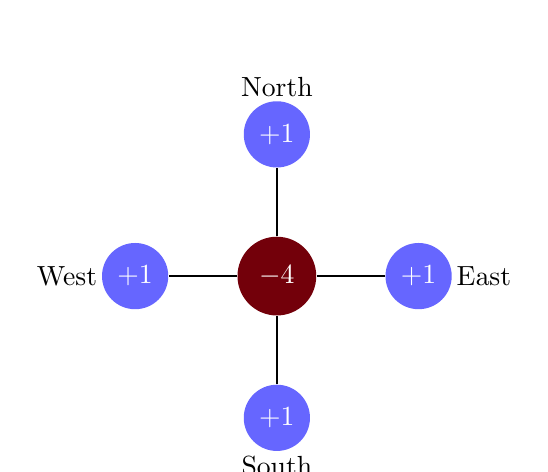
\begin{tikzpicture}[scale=1.2]
    % Center node
    \node[circle, fill=USC_Garnet, text=white, minimum size=1cm] (C) at (0,0) {$-4$};
    % Neighbor nodes
    \node[circle, fill=blue!60, text=white, minimum size=0.8cm] (E) at (1.5,0) {$+1$};
    \node[circle, fill=blue!60, text=white, minimum size=0.8cm] (W) at (-1.5,0) {$+1$};
    \node[circle, fill=blue!60, text=white, minimum size=0.8cm] (N) at (0,1.5) {$+1$};
    \node[circle, fill=blue!60, text=white, minimum size=0.8cm] (S) at (0,-1.5) {$+1$};
    % Lines
    \draw[thick] (C) -- (E); \draw[thick] (C) -- (W);
    \draw[thick] (C) -- (N); \draw[thick] (C) -- (S);
    % Labels
    \node[right] at (1.8,0) {East};
    \node[left] at (-1.8,0) {West};
    \node[above] at (0,1.8) {North};
    \node[below] at (0,-1.8) {South};
\end{tikzpicture}
\end{center}
\end{resultsbox}


% ============================================================================
% PROBLEM 1: Exercise 15.1 Problem 7 - Part (b)
% ============================================================================

\questionpart{Exercise 15.1: Problem 7 --- Part (b)}\label{quest:1b}

\textbf{(b)} Use the result in part (a) to approximate the solution of the Poisson equation
\[
\frac{\partial^2 u}{\partial x^2} + \frac{\partial^2 u}{\partial y^2} = -2
\]
at the interior points of the region in Figure 15.1.7. The mesh size is $h = \dfrac{1}{2}$, $u = 1$ at every point along $ABCD$, and $u = 0$ at every point along $DEFGA$. \underline{Use symmetry} and, if necessary, Gauss-Seidel iteration.

\vspace{0.5cm}
\begin{center}
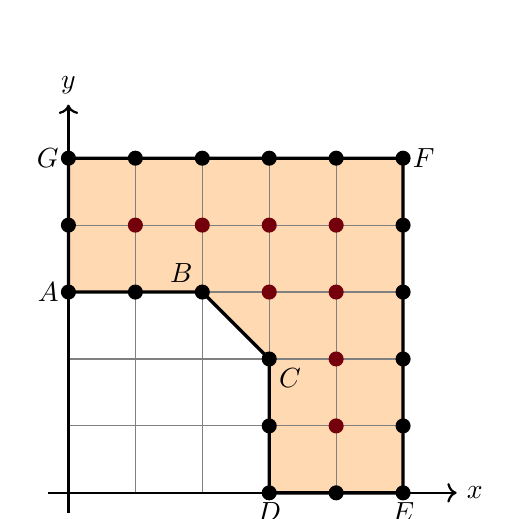
\begin{tikzpicture}[scale=0.85]
    % Fill the L-shaped region
    \fill[orange!30] (3,0) -- (5,0) -- (5,5) -- (0,5) -- (0,3) -- (2,3) -- (3,2) -- cycle;
    
    % Draw grid lines
    \foreach \x in {0,1,2,3,4,5} {
        \draw[gray, thin] (\x, 0) -- (\x, 5);
    }
    \foreach \y in {0,1,2,3,4,5} {
        \draw[gray, thin] (0, \y) -- (5, \y);
    }
    
    % Draw axes
    \draw[->,thick] (-0.3,0) -- (5.8,0) node[right] {$x$};
    \draw[->,thick] (0,-0.3) -- (0,5.8) node[above] {$y$};
    
    % Draw boundary outline (thick black line)
    \draw[very thick] (3,0) -- (5,0) -- (5,5) -- (0,5) -- (0,3) -- (2,3) -- (3,2) -- cycle;
    
    % Interior points (USC Garnet)
    \foreach \x in {1, 2, 3, 4} {
        \fill[USC_Garnet] (\x, 4) circle (3.2pt);
    }
    \foreach \x in {3, 4} {
        \fill[USC_Garnet] (\x, 3) circle (3.2pt);
    }
    \fill[USC_Garnet] (4, 2) circle (3.2pt);
    \fill[USC_Garnet] (4, 1) circle (3.2pt);
    
    % Boundary points (black)
    \foreach \x in {3, 4, 5} {
        \fill[black] (\x, 0) circle (3.2pt);
    }
    \foreach \y in {1, 2, 3, 4, 5} {
        \fill[black] (5, \y) circle (3.2pt);
    }
    \foreach \x in {0, 1, 2, 3, 4} {
        \fill[black] (\x, 5) circle (3.2pt);
    }
    \foreach \y in {3, 4} {
        \fill[black] (0, \y) circle (3.2pt);
    }
    \foreach \x in {1, 2} {
        \fill[black] (\x, 3) circle (3.2pt);
    }
    \foreach \y in {1, 2} {
        \fill[black] (3, \y) circle (3.2pt);
    }
    
    % Labels for boundary corners
    \node[left] at (0, 3) {$A$};
    \node[above left] at (2, 3) {$B$};
    \node[below right] at (3, 2) {$C$};
    \node[below] at (3, 0) {$D$};
    \node[below] at (5, 0) {$E$};
    \node[right] at (5, 5) {$F$};
    \node[left] at (0, 5) {$G$};
    
\end{tikzpicture}

\textbf{FIGURE 15.1.7} Region for Problem 7
\end{center}

\begin{stepbox}
\textbf{Problem Setup}

For $f(x,y) = -2$ and $h = 1/2$, the difference equation becomes:
\[
u_{i+1,j} + u_{i,j+1} + u_{i-1,j} + u_{i,j-1} - 4u_{i,j} = \left(\frac{1}{2}\right)^2 \cdot (-2) = -\frac{1}{2}
\]

\textbf{Boundary conditions:}
\begin{itemize}
    \item $u = 1$ along $ABCD$ (the stair-step inner boundary)
    \item $u = 0$ along $DEFGA$ (the outer boundary: bottom, right, and top)
\end{itemize}

\textbf{Identifying Interior Points:} Using the grid with $h = 0.5$, there are 6 interior points. Due to diagonal symmetry about $y = x$:
\[
u_1 = u_6, \quad u_2 = u_5
\]
This reduces the problem to \textbf{4 unknowns}: $u_1, u_2, u_3, u_4$.
\end{stepbox}

\begin{codebox}
\begin{lstlisting}
import numpy as np

# Problem parameters
h = 0.5   # mesh size
f = -2    # source term
rhs = h**2 * f  # = -0.5

# System using symmetry: [u1, u2, u3, u4]
A = np.array([
    [-4,  1,  0,  0],   # Eq 1: -4u1 + u2 = -1.5
    [ 1, -4,  1,  1],   # Eq 2: u1 - 4u2 + u3 + u4 = -0.5
    [ 0,  2, -4,  0],   # Eq 3: 2u2 - 4u3 = -0.5
    [ 0,  2,  0, -4]    # Eq 4: 2u2 - 4u4 = -2.5
], dtype=float)

b = np.array([-1.5, -0.5, -0.5, -2.5])

# Solve directly
u = np.linalg.solve(A, b)
print("Direct Method Solution:")
for i, val in enumerate(u, 1):
    print(f"  u{i} = {val:.6f}")
\end{lstlisting}
\end{codebox}

\begin{outputbox}
\begin{lstlisting}[style=output]
SOLUTION (Direct Method):
--------------------------------------------------

  u1 = u6 = 0.522727  (exact: 23/44 = 0.522727)
  u2 = u5 = 0.590909  (exact: 13/22 = 0.590909)
  u3      = 0.420455  (exact: 37/88 = 0.420455)
  u4      = 0.920455  (exact: 81/88 = 0.920455)

GAUSS-SEIDEL ITERATION
==================================================

Initial guess: u = [0.5000, 0.5000, 0.5000, 0.5000]
Convergence tolerance: 1e-08

 Iter         u1         u2         u3         u4       Max du
------------------------------------------------------------
    1   0.500000   0.500000   0.375000   0.875000     3.75e-01
    2   0.500000   0.562500   0.406250   0.906250     6.25e-02
    3   0.515625   0.582031   0.416016   0.916016     1.95e-02
    4   0.520508   0.588135   0.419067   0.919067     6.10e-03
    5   0.522034   0.590042   0.420021   0.920021     1.91e-03
    ...
   16   0.522727   0.590909   0.420455   0.920455     5.29e-09

Converged after 16 iterations!
\end{lstlisting}
\end{outputbox}

\begin{resultsbox}
\textbf{Final Solution:}

\begin{center}
\begin{tabular}{c|c|c|c}
\toprule
Point & Location $(x, y)$ & Value $u$ & Exact Fraction \\
\midrule
$u_1$ & $(0.5, 1.5)$ & $0.5227$ & $23/44$ \\
$u_2$ & $(1.0, 1.5)$ & $0.5909$ & $13/22$ \\
$u_3$ & $(1.5, 1.5)$ & $0.4205$ & $37/88$ \\
$u_4$ & $(1.0, 1.0)$ & $0.9205$ & $81/88$ \\
$u_5$ & $(1.5, 1.0)$ & $0.5909$ & $13/22$ \\
$u_6$ & $(1.5, 0.5)$ & $0.5227$ & $23/44$ \\
\bottomrule
\end{tabular}
\end{center}

The Gauss-Seidel method converges in \textbf{16 iterations} to within $10^{-8}$ tolerance, demonstrating excellent convergence for this well-conditioned problem.
\end{resultsbox}

\begin{figure}[H]
\centering
\includegraphics[width=0.95\textwidth]{poisson_solution.png}
\caption{Left: L-shaped domain with computed interior point values. Right: Solution heatmap showing the potential distribution.}
\label{fig:poisson_solution}
\end{figure}


% ============================================================================
% PROBLEM 2: Exercise 15.2 Problem 10 - Part (a)
% ============================================================================

\questionpart{Exercise 15.2: Problem 10 --- Part (a) (20 pts)}\label{quest:2a}

Consider the boundary-value problem from Example 2:
\begin{align*}
0.25\frac{\partial^2 u}{\partial x^2} &= \frac{\partial u}{\partial t}, \quad 0 < x < 2, \quad 0 < t < 0.3\\
u(0,t) &= 0, \quad u(2,t) = 0, \quad 0 \leq t \leq 0.3\\
u(x,0) &= \sin(\pi x), \quad 0 \leq x \leq 2
\end{align*}
using $n = 4$, $m = 30$.

\vspace{0.3cm}
\textbf{(a)} Find $\lambda$

\begin{stepbox}
\textbf{Step 1: Identify Parameters}

The PDE is $0.25 u_{xx} = u_t$, which can be written as $u_t = k u_{xx}$ where:
\begin{itemize}
    \item $k = 0.25$ is the thermal diffusivity
    \item Domain: $x \in [0, 2]$, $t \in [0, 0.3]$
\end{itemize}

\textbf{Spatial discretization:} With $n = 4$ divisions over $[0, 2]$:
\[
h = \frac{L}{n} = \frac{2}{4} = 0.5
\]

\textbf{Temporal discretization:} With $m = 30$ divisions over $[0, 0.3]$:
\[
\Delta t = \frac{T}{m} = \frac{0.3}{30} = 0.01
\]
\end{stepbox}

\begin{stepbox}
\textbf{Step 2: Compute $\lambda$}

The stability parameter $\lambda$ for the heat equation is defined as:
\[
\lambda = \frac{k \Delta t}{h^2}
\]

Substituting our values:
\[
\lambda = \frac{0.25 \times 0.01}{(0.5)^2} = \frac{0.0025}{0.25} = 0.01
\]
\end{stepbox}

\begin{resultsbox}
\[
\boxed{\lambda = 0.01}
\]

\textbf{Note:} This small value of $\lambda$ indicates that the time step is much smaller than the stability limit ($\lambda \leq 0.5$ for explicit methods). The Crank-Nicholson method is unconditionally stable for any $\lambda > 0$.
\end{resultsbox}


% ============================================================================
% PROBLEM 2: Exercise 15.2 Problem 10 - Part (b)
% ============================================================================

\questionpart{Exercise 15.2: Problem 10 --- Part (b)}\label{quest:2b}

\textbf{(b)} Use the Crank-Nicholson difference equation
\[
-u_{i-1,j+1} + \alpha u_{i,j+1} - u_{i+1,j+1} = u_{i+1,j} - \beta u_{i,j} + u_{i-1,j}
\]
where $\alpha = 2(1 + 1/\lambda)$ and $\beta = 2(1 - 1/\lambda)$, to find the system of equations for $u_{1,1}$, $u_{2,1}$ and $u_{3,1}$.

\begin{stepbox}
\textbf{Step 1: Compute $\alpha$ and $\beta$}

With $\lambda = 0.01$:
\[
\alpha = 2\left(1 + \frac{1}{\lambda}\right) = 2\left(1 + \frac{1}{0.01}\right) = 2(1 + 100) = \boxed{202}
\]
\[
\beta = 2\left(1 - \frac{1}{\lambda}\right) = 2\left(1 - 100\right) = 2(-99) = \boxed{-198}
\]

Note: On the RHS of the difference equation, we have $-\beta u_{i,j}$, which becomes $-(-198)u_{i,j} = +198 u_{i,j}$.
\end{stepbox}

\begin{stepbox}
\textbf{Step 2: Initial Conditions}

At $t = 0$, $u(x, 0) = \sin(\pi x)$ with grid points $x_i = i \cdot h = 0.5i$:
\begin{align*}
u_{0,0} &= \sin(0) = 0 \\
u_{1,0} &= \sin(0.5\pi) = 1 \\
u_{2,0} &= \sin(\pi) = 0 \\
u_{3,0} &= \sin(1.5\pi) = -1 \\
u_{4,0} &= \sin(2\pi) = 0
\end{align*}

\textbf{Boundary conditions:} $u_{0,j} = 0$ and $u_{4,j} = 0$ for all $j$.
\end{stepbox}

\begin{stepbox}
\textbf{Step 3: Write Equations for $j = 0$ (First Time Step)}

The Crank-Nicholson equation becomes:
\[
-u_{i-1,j+1} + 202 u_{i,j+1} - u_{i+1,j+1} = u_{i+1,j} + 198 u_{i,j} + u_{i-1,j}
\]

\textbf{For $i = 1$:}
\begin{align*}
-u_{0,1} + 202u_{1,1} - u_{2,1} &= u_{2,0} + 198u_{1,0} + u_{0,0} \\
-0 + 202u_{1,1} - u_{2,1} &= 0 + 198(1) + 0 \\
\Rightarrow \quad 202u_{1,1} - u_{2,1} &= 198
\end{align*}

\textbf{For $i = 2$:}
\begin{align*}
-u_{1,1} + 202u_{2,1} - u_{3,1} &= u_{3,0} + 198u_{2,0} + u_{1,0} \\
-u_{1,1} + 202u_{2,1} - u_{3,1} &= -1 + 0 + 1 \\
\Rightarrow \quad -u_{1,1} + 202u_{2,1} - u_{3,1} &= 0
\end{align*}

\textbf{For $i = 3$:}
\begin{align*}
-u_{2,1} + 202u_{3,1} - u_{4,1} &= u_{4,0} + 198u_{3,0} + u_{2,0} \\
-u_{2,1} + 202u_{3,1} - 0 &= 0 + 198(-1) + 0 \\
\Rightarrow \quad -u_{2,1} + 202u_{3,1} &= -198
\end{align*}
\end{stepbox}

\begin{resultsbox}
\textbf{System of Equations:}
\begin{align*}
202u_{1,1} - u_{2,1} &= 198 \\
-u_{1,1} + 202u_{2,1} - u_{3,1} &= 0 \\
-u_{2,1} + 202u_{3,1} &= -198
\end{align*}

In matrix form:
\[
\begin{pmatrix}
202 & -1 & 0 \\
-1 & 202 & -1 \\
0 & -1 & 202
\end{pmatrix}
\begin{pmatrix}
u_{1,1} \\
u_{2,1} \\
u_{3,1}
\end{pmatrix}
=
\begin{pmatrix}
198 \\
0 \\
-198
\end{pmatrix}
\]

This is a \textbf{tridiagonal system} which can be solved efficiently using the Thomas algorithm.
\end{resultsbox}


% ============================================================================
% PROBLEM 2: Exercise 15.2 Problem 10 - Part (c)
% ============================================================================

\questionpart{Exercise 15.2: Problem 10 --- Part (c)}\label{quest:2c}

\textbf{(c)} Solve the system of three equations \underline{without} the aid of a computer program.

\begin{stepbox}
\textbf{Using Symmetry}

From the initial condition $u(x, 0) = \sin(\pi x)$, we observe the antisymmetry property:
\[
\sin(\pi(2-x)) = \sin(2\pi - \pi x) = -\sin(\pi x)
\]

This antisymmetry about $x = 1$ is preserved by the heat equation. Therefore:
\begin{itemize}
    \item $u_{1,j} = -u_{3,j}$ for all $j$ (antisymmetric points)
    \item $u_{2,j} = 0$ for all $j$ (center point on axis of antisymmetry)
\end{itemize}
\end{stepbox}

\begin{stepbox}
\textbf{Solving Using Symmetry}

Let $u_{1,1} = -u_{3,1}$ and $u_{2,1} = 0$.

From equation (1): $202u_{1,1} - u_{2,1} = 198$
\[
202u_{1,1} - 0 = 198 \implies u_{1,1} = \frac{198}{202} = \frac{99}{101}
\]

Therefore:
\[
u_{3,1} = -u_{1,1} = -\frac{99}{101}
\]
\end{stepbox}

\begin{stepbox}
\textbf{Verification}

\textbf{Check equation (2):} $-u_{1,1} + 202u_{2,1} - u_{3,1} = 0$
\[
-\frac{99}{101} + 202(0) - \left(-\frac{99}{101}\right) = -\frac{99}{101} + \frac{99}{101} = 0 \quad \checkmark
\]

\textbf{Check equation (3):} $-u_{2,1} + 202u_{3,1} = -198$
\[
-0 + 202\left(-\frac{99}{101}\right) = -\frac{202 \times 99}{101} = -\frac{2 \times 99}{1} = -198 \quad \checkmark
\]
\end{stepbox}

\begin{resultsbox}
\textbf{Solutions:}
\[
u_{1,1} = \frac{99}{101} \approx \boxed{0.9802}
\]
\[
u_{2,1} = \boxed{0}
\]
\[
u_{3,1} = -\frac{99}{101} \approx \boxed{-0.9802}
\]
\end{resultsbox}

\begin{outputbox}
\begin{lstlisting}[style=output]
FULL TIME EVOLUTION (Crank-Nicholson)
==================================================

Solution at selected times (coarse grid h=0.5):
-----------------------------------------------------------------
       t | x=0.00 | x=0.50 | x=1.00 | x=1.50 | x=2.00 |
-----------------------------------------------------------------
   0.000 | 0.0000 | 1.0000 | 0.0000 | -1.0000 | -0.0000 |
   0.010 | 0.0000 | 0.9802 | 0.0000 | -0.9802 | 0.0000 |
   0.050 | 0.0000 | 0.9048 | 0.0000 | -0.9048 | 0.0000 |
   0.100 | 0.0000 | 0.8187 | 0.0000 | -0.8187 | 0.0000 |
   0.150 | 0.0000 | 0.7408 | 0.0000 | -0.7408 | 0.0000 |
   0.200 | 0.0000 | 0.6703 | 0.0000 | -0.6703 | 0.0000 |
   0.300 | 0.0000 | 0.5488 | 0.0000 | -0.5488 | 0.0000 |
\end{lstlisting}
\end{outputbox}

\begin{figure}[H]
\centering
\includegraphics[width=0.95\textwidth]{crank_nicholson_evolution.png}
\caption{Left: Temperature profiles at different times showing antisymmetric decay. Right: Heatmap of the full space-time evolution.}
\label{fig:crank_nicholson}
\end{figure}


% ============================================================================
% PROBLEM 3: Exercise 15.2 Problem 12
% ============================================================================

\questionpart{Exercise 15.2: Problem 12 (25 pts)}\label{quest:3}

Use the difference equation
\[
u_{i,j+1} = \lambda u_{i+1,j} + (1 - 2\lambda)u_{i,j} + \lambda u_{i-1,j}
\]
to approximate the solution of the boundary-value problem
\begin{align*}
\frac{\partial^2 u}{\partial x^2} &= \frac{\partial u}{\partial t}, \quad 0 < x < 1, \quad 0 < t < 1\\
u(0,t) &= 0, \quad u(1,t) = 0, \quad 0 \leq t \leq 1\\
u(x,0) &= x(1-x), \quad 0 \leq x \leq 1
\end{align*}

Use $n = 5$ and $m = 50$. \textbf{Solve this using Python.}

\begin{stepbox}
\textbf{Step 1: Grid Parameters}

\textbf{Spatial discretization:} With $n = 5$ divisions over $[0, 1]$:
\[
h = \frac{1}{n} = \frac{1}{5} = 0.2
\]

\textbf{Temporal discretization:} With $m = 50$ divisions over $[0, 1]$:
\[
\Delta t = \frac{1}{m} = \frac{1}{50} = 0.02
\]

\textbf{Stability parameter:} For the heat equation $u_t = u_{xx}$ (diffusivity $k = 1$):
\[
\lambda = \frac{k \Delta t}{h^2} = \frac{1 \times 0.02}{(0.2)^2} = \frac{0.02}{0.04} = \boxed{0.5}
\]

\textbf{Stability:} The explicit method is stable when $\lambda \leq 0.5$. We are exactly at the stability limit!
\end{stepbox}

\begin{stepbox}
\textbf{Step 2: Initial and Boundary Conditions}

\textbf{Initial condition} at $t = 0$: $u(x, 0) = x(1-x)$

\begin{center}
\begin{tabular}{c|cccccc}
$i$ & 0 & 1 & 2 & 3 & 4 & 5 \\
\hline
$x_i$ & 0 & 0.2 & 0.4 & 0.6 & 0.8 & 1.0 \\
$u_{i,0}$ & 0 & 0.16 & 0.24 & 0.24 & 0.16 & 0
\end{tabular}
\end{center}

\textbf{Boundary conditions:} $u_{0,j} = 0$ and $u_{5,j} = 0$ for all $j$.
\end{stepbox}

\begin{stepbox}
\textbf{Step 3: Explicit Update Formula}

With $\lambda = 0.5$, the difference equation simplifies dramatically:
\[
u_{i,j+1} = 0.5 \cdot u_{i+1,j} + (1 - 1) \cdot u_{i,j} + 0.5 \cdot u_{i-1,j}
\]
\[
\boxed{u_{i,j+1} = \frac{1}{2}(u_{i+1,j} + u_{i-1,j})}
\]

This is simply the \textbf{average of the neighboring values}! The center point's current value has zero weight.
\end{stepbox}

\begin{codebox}
\begin{lstlisting}
import numpy as np
import matplotlib.pyplot as plt

# Parameters
L = 1.0; T_final = 1.0
n = 5; m = 50
h = L / n        # h = 0.2
dt = T_final / m # dt = 0.02
lam = dt / h**2  # lambda = 0.5

# Grid
x = np.linspace(0, L, n+1)
t = np.linspace(0, T_final, m+1)

# Initialize solution
u = np.zeros((m+1, n+1))
u[0, :] = x * (1 - x)  # Initial condition

# Time stepping (explicit method)
for j in range(m):
    for i in range(1, n):
        u[j+1, i] = lam*u[j,i+1] + (1-2*lam)*u[j,i] + lam*u[j,i-1]

# Print results
print("Solution at selected times:")
for j in [0, 10, 20, 30, 40, 50]:
    print(f"t={t[j]:.2f}: ", [f"{u[j,i]:.4f}" for i in range(n+1)])
\end{lstlisting}
\end{codebox}

\begin{outputbox}
\begin{lstlisting}[style=output]
STEP 4: First Few Time Steps (Manual)
----------------------------------------
  j = 0 -> j = 1 (t = 0.00 -> t = 0.02):
    u_{1,1} = 0.5 x (0.2400 + 0.0000) = 0.1200
    u_{2,1} = 0.5 x (0.2400 + 0.1600) = 0.2000
    u_{3,1} = 0.5 x (0.1600 + 0.2400) = 0.2000
    u_{4,1} = 0.5 x (0.0000 + 0.2400) = 0.1200

  j = 1 -> j = 2 (t = 0.02 -> t = 0.04):
    u_{1,2} = 0.5 x (0.2000 + 0.0000) = 0.1000
    u_{2,2} = 0.5 x (0.2000 + 0.1200) = 0.1600
    u_{3,2} = 0.5 x (0.1200 + 0.2000) = 0.1600
    u_{4,2} = 0.5 x (0.0000 + 0.2000) = 0.1000

NUMERICAL RESULTS
=================================================================
       t | x=0.0 | x=0.2 | x=0.4 | x=0.6 | x=0.8 | x=1.0 |
-----------------------------------------------------------------
    0.00 | 0.0000 | 0.1600 | 0.2400 | 0.2400 | 0.1600 | 0.0000 |
    0.20 | 0.0000 | 0.0182 | 0.0295 | 0.0295 | 0.0182 | 0.0000 |
    0.40 | 0.0000 | 0.0022 | 0.0035 | 0.0035 | 0.0022 | 0.0000 |
    0.60 | 0.0000 | 0.0003 | 0.0004 | 0.0004 | 0.0003 | 0.0000 |
    0.80 | 0.0000 | 0.0000 | 0.0001 | 0.0001 | 0.0000 | 0.0000 |
    1.00 | 0.0000 | 0.0000 | 0.0000 | 0.0000 | 0.0000 | 0.0000 |
\end{lstlisting}
\end{outputbox}

\begin{resultsbox}
\textbf{Observations:}
\begin{enumerate}
    \item \textbf{Symmetry:} The solution maintains symmetry about $x = 0.5$ throughout, reflecting the symmetric initial condition.
    \item \textbf{Decay:} The temperature decays exponentially toward zero (the boundary values).
    \item \textbf{Maximum:} The peak temperature is always at the center ($x = 0.5$).
    \item \textbf{Stability:} With $\lambda = 0.5$ at the stability limit, the method remains stable and provides smooth results.
\end{enumerate}

\textbf{Energy Decay:}
\begin{center}
\begin{tabular}{c|c}
\toprule
$t$ & Total Energy $\int_0^1 u^2 \, dx$ \\
\midrule
0.00 & 0.033280 \\
0.20 & 0.000480 \\
0.40 & 0.000007 \\
\bottomrule
\end{tabular}
\end{center}

The energy decays by approximately three orders of magnitude every 0.2 time units.
\end{resultsbox}

\begin{figure}[H]
\centering
\includegraphics[width=0.85\textwidth]{heat_explicit_evolution.png}
\caption{Temperature profiles at different times showing exponential decay from the initial parabolic distribution $u(x,0) = x(1-x)$.}
\label{fig:heat_evolution}
\end{figure}

\begin{figure}[H]
\centering
\includegraphics[width=0.85\textwidth]{heat_explicit_surface.png}
\caption{3D surface plot of the heat equation solution $u(x,t)$ showing the complete spatiotemporal evolution.}
\label{fig:heat_surface}
\end{figure}

\begin{figure}[H]
\centering
\includegraphics[width=0.95\textwidth]{heat_explicit_heatmap.png}
\caption{Heatmap representation of the temperature evolution. The rapid decay from the initial condition is clearly visible.}
\label{fig:heat_heatmap}
\end{figure}

\begin{outputbox}
\begin{lstlisting}[style=output]
ANALYTICAL SOLUTION COMPARISON
----------------------------------------
  Exact solution (Fourier series):
    u(x,t) = Sum B_n sin(n*pi*x) exp(-n^2*pi^2*t)

  where B_n = (2/L) integral_0^1 x(1-x) sin(n*pi*x) dx

  For odd n: B_n = 8/(n^3*pi^3)
  For even n: B_n = 0

  Comparison at x = 0.5:
         t    Numerical   Analytical        Error
  ------------------------------------------------
      0.00     0.240000     0.250000     1.00e-02
      0.20     0.029453     0.035841     6.39e-03
      0.40     0.003538     0.004979     1.44e-03
      0.60     0.000425     0.000692     2.67e-04
      0.80     0.000051     0.000096     4.50e-05
      1.00     0.000006     0.000013     7.22e-06
\end{lstlisting}
\end{outputbox}

\begin{figure}[H]
\centering
\includegraphics[width=0.95\textwidth]{heat_explicit_comparison.png}
\caption{Left: Comparison of numerical (markers) and analytical (lines) solutions at different times. Right: Error decay at the center point $x = 0.5$.}
\label{fig:heat_comparison}
\end{figure}


% ============================================================================
% END OF DOCUMENT
% ============================================================================

\end{document}
